% !TeX root = ../../book.tex
\section{集合}
\secbegin{secSets}
\index{set|(}

我们首先重新定义\textit{集合}的概念，其精度比我们在 \Cref{chGettingStarted} 中给出的精度更高。从本质上讲，集合看起来非常简单 --- 集合只是对象的汇集 --- 但如果不加以控制，集合的这种特性会导致逻辑上的不一致，例如臭名昭著的\textit{罗素悖论}。

这些逻辑悖论可以通过将我们的工作限制在\textit{全集} $\mathcal{U}$ 内来克服，我们认为这个全集是一个非常大的集合，包含了我们想要讨论的所有数学对象。这是一个微妙的问题，远远超出本节的范围，但会在 \Cref{secZFC} 中进一步讨论。

\begin{definition}
\label{defSet}
\index{set}
\index{element}
\index{universal set}
\index{universe!of discourse}
\textbf{集合}\index{set}是来自指定\textbf{论域}\index{universe of discourse}的\textbf{元素}的汇集。论域中所有事物的汇集称为\textbf{全集}\index{set!universal}，写做 $\mathcal{U}$\nindex{U}{$\mathcal{U}$}{全集} \inlatex{mathcal\{U\}}\lindexmmc{mathcal}{$\mathcal{A}, \mathcal{B}, \dots$}。

表达式 $x \in X$\nindex{in}{$\in$}{元素} \inlatex{in}\lindexmmc{in}{$\in$} 表示 $x$ 是 $X$ 的元素；$x \not \in X$ \inlatex{not\textbackslash{}in}\lindexmmc{not}{$\not\in, \not\equiv, \dots$} 表示 $\neg (x \in X)$，即 $x$ 不是 $X$ 的元素。
\end{definition}

\begin{example}
在\Cref{chGettingStarted}中，我们引入了五个集合：自然数集合 $\mathbb{N}$、整数集合 $\mathbb{Z}$、有理数集合 $\mathbb{Q}$，实数集合 $\mathbb{R}$ 和复数集合 $\mathbb{C}$。
\end{example}

\begin{exercise}
以下命题哪些是正确的，哪些是错误的？
\[ \frac{1}{2} \in \mathbb{Z} \qquad \frac{1}{2} \in \mathbb{Q} \qquad \mathbb{Z} \in \mathbb{Q} \qquad \mathbb{Z} \in \mathcal{U} \qquad \frac{1}{2} \in \mathcal{U} \]
\hintlabel{exElementsOfSets}{%
想一想 `$a \in X$' \textit{真正的含义}是什么 --- 不要让直觉欺骗了你。
}
\end{exercise}

我们尽可能避免显式引用全集 $\mathcal{U}$，但它始终存在于背后。这样会很方便，因为我们不再需要担心自由变量的论域（就像我们在 \Cref{defPredicate} 中所做的那样），因此我们可以将 `$\forall x \in \mathcal{U},\, p(x)$' 缩写成 `$\forall x,\, p(x)$'，并且将 `$\exists x \in \mathcal{U},\, p(x)$' 缩写成 `$\exists x ,\,p(x)$'。

请注意，根据该约定：
\begin{itemize}
\item $\forall x \in X,\, p(x)$ 逻辑等价于 $\forall x,\, (x \in X \Rightarrow p(x))$；
\item $\exists x \in X,\, p(x)$ 逻辑等价于 $\exists x,\, (x \in X \wedge p(x))$。
\end{itemize}

\subsection*{指定一个集合}
定义集合的一种方法就是简单地用文字描述它，就像我们到之前所做的那样。当然还有其他更简洁的方法，这些方法也可以消除过程中的某些歧义。

\textbf{列表}\index{list notation}
一种方法是简单地提供集合元素的\textbf{列表}。为了表明列表表示一个集合，我们用 $\{$ 大括号 $\}$\nindex{set}{$\{ \cdots \}$}{set notation} \inlatex{\{,\textbackslash{}\}}\lindexmmc{\{\dots\textbackslash{}\}}{$\{\dots\}$} 将列表括起来。 例如，下面指定了一个集合 $X$，其元素是 $0$ 到 $5$（含）之间的自然数：
\[ X = \{ 0, 1, 2, 3, 4, 5 \} \]

\textbf{隐式列表}\index{implied list notation}
有时列表可能太长而无法写出 --- 甚至可能是无限的 --- 或者列表的长度取决于变量。在这些情况下，使用\textbf{隐式列表}会很更方便，其中写入列表的某些元素，并通过省略号 `$\dots$' \inlatex{dots}\lindexmmc{dots}{ $\dots$} 来隐式保留其余元素 。 例如，
\[ X = \{ 1, 4, 9, \dots, n^2 \} \]
表示 $X$ 是一个集合，其元素是 $1$ 到 $n^2$ 之间的所有平方数，其中 $n$ 是某个数字。隐式列表可能不明确，因为它依赖读者推断遵循模式的能力，因此请谨慎使用！

\textbf{集合构建表示法}\index{set-builder notation}
一般来说，隐式列表可能是不明确的，因此在实践中应避免使用它们，除非隐式列表非常简单，例如一组连续的数字，如 $\{3, 4, \dots, 9 \}$。事实上，很多集合无法以这种方式给出。

为了解决这个问题，我们可以使用\textit{集合构建表示法}，这是一种根据集合元素满足的属性来指定集合的方法。给定一个集合 $X$, $X$ 满足某些属性 $p(x)$ 的元素集合表示为
\[ \{ x \in X \mid p(x) \} \]
竖线 `$\mid$' \inlatex{mid}\lindexmmc{mid}{$\mid$} 将变量名与它所在的公式分开 --- 一些作者会用冒号代替（如 $\{ x \in X : p(x) \}$）。

集合 $\{ x \in X \mid p(x) \}$ 读作 `$x \in X$ 使得 $p(x)$ 的集合'，但是要注意 --- 无论是竖线 `$\mid$' 还是冒号 `$:$' 在其他场景中均表示`使得'。

\begin{example}
\label{exSetsSpecifyUniverses}
所有偶数的集合可以用集合构建表示法写为
\[ \{ n \in \mathbb{Z} \mid n \text{为偶数} \} \]
为了比较，所有偶自然数的集合可以写为
\[ \{ n \in \mathbb{N} \mid n \text{为偶数} \} = \{ 0, 2, 4, 6, \dots \} \]
请注意，$-6$ 是前一个集合的元素，但不是后一个集合的元素，因为 $-6$ 是整数但不是自然数。

此外还请注意，表达式
\[ \{ n \in \mathbb{Q} \mid n \text{为偶数} \} \]
是没有意义的，因为我们没有为有理数定义 `奇偶' 的概念。
\end{example}

\begin{strategy}
设$X$ 为集合，$p(x)$ 为带有自由变量 $x \in X$ 的逻辑公式。为了证明 $a \in \{ x \in X \mid p(x) \}$，只需证明 $a \in X$ 且 $p(a)$ 为真。
\end{strategy}

\begin{exercise}
\label{exDyadicRatioal}
\index{rational number!dyadic}
\textbf{二进有理数} 指分母为 $2$ 的幂分子为整数的有理数。使用集合构建表示法表示出所有二进有理数的集合。
\end{exercise}

集合构建表示法的另一种形式是将包含一个或多个变量的表达式放在竖线左侧，变量的取值范围放在竖线右侧。当变量按指示变化时，集合的元素就是表达式的值，即：
\[ \{ \mathsf{expr}(x) \mid x \in X \} \text{意味着} \{ y \mid \exists x \in X,\, y = \mathsf{expr}(x) \} \]
其中 $\mathsf{expr}(x)$ 是表达式。

\begin{example}
表达式 $\{ 3k+2 \mid k \in \mathbb{Z} \}$ 表示 $3k+2$ 形式的所有整数的集合，其中 $k \in \mathbb{Z}$。它是 $\{ n \in \mathbb{Z} \mid \exists k \in \mathbb{Z},\, n=3k+2 \}$ 的简写。在隐式列表表示法中，我们可以将这个集合写为 $\{ \dots, {-4}, {-1}, 2, 5, 8, \dots \}$。
\end{example}

\begin{exercise}
用集合构建表示法的替代形式表达二进有理数集（在 \Cref{exDyadicRatioal} 中定义）。
\end{exercise}

集合构建表示法对于根据集合满足的属性定义集合非常有用，如下面的 \Cref{defBracketN,defIntervals} 所示。

\begin{restatable}{definition}{RSdefBracketN}
\label{defBracketN}
设 $n \in \mathbb{N}$。集合 $[n]$ 定义为 $[n] = \{ k \in \mathbb{N} \mid 1 \le k \le n \}$。
\end{restatable}

\begin{example}
\label{exBracketN}
在隐式列表表示法中，$[n] = \{ 1, 2, \dots, n \}$。例如，$[4] = \{ 1, 2, 3, 4 \}$。注意 $[0]$ 没有元素（它是 \textit{空集} --- 参见 \Cref{defInhabited}），因为不存在满足不等式 $1 \le k \le 0$ 的自然数 $k$。
\end{example}

虽然还不是特别有趣，但 $[n]$ 形式的集合将是整个 \Cref{chCombinatorics} 的基础，因为它们用于定义\textit{有限集}的概念，以及有限集的\textit{大小} 。

区间是 $\mathbb{R}$ 的特定子集，在数学中普遍存在，特别是在分析和拓扑中。

\begin{definition}[实数的区间]
\label{defIntervals}
\index{interval!open}
\index{interval!closed}
\index{interval!half-open}
\index{open!interval}
\index{closed!interval}
\nindex{abint1}{$(a,b)$}{open interval}
\nindex{abint2}{$[a,b]$}{closed interval}
\nindex{abint3}{$(a,b]$}{half-open interval}
\nindex{abint4}{$[a,b)$}{half-open interval}
\nindex{abint5}{$(-\infty,a)$}{unbounded interval}
\nindex{abint6}{$(a,\infty)$}{unbounded interval}
设 $a,b \in \mathbb{R}$。\textbf{开区间} $(a,b)$、\textbf{闭区间} $[a,b]$ 以及 \textbf{半开区间} $[a,b)$ 和 $( a,b]$ 从 $a$ 到 $b$ 定义为
\begin{align*}
\hspace{35pt} (a,b) &= \{ x \in \mathbb{R} \mid a < x < b \}
&
(a,b] &= \{ x \in \mathbb{R} \mid a < x \le b \} 
\\
\hspace{35pt} [a,b) &= \{ x \in \mathbb{R} \mid a \le x < b \}
&
[a,b] &= \{ x \in \mathbb{R} \mid a \le x \le b \}
\end{align*}
我们进一步定义\textbf{无界区间} $(-\infty, a)$, $(-\infty, a]$, $[a, \infty)$ 和 $(a, \infty)$ \inlatex{infty}\lindexmmc{infty}{$\infty$}
\begin{align*}
\hspace{35pt} (-\infty,a) &= \{ x \in \mathbb{R} \mid x < a \}
&
(a,\infty) &= \{ x \in \mathbb{R} \mid x > a \}
\\
\hspace{35pt} (-\infty, a] &= \{ x \in \mathbb{R} \mid x \le a \} 
&
[a,\infty) &= \{ x \in \mathbb{R} \mid x \ge a \}
\end{align*}
\end{definition}

\begin{example}
下图描述了开区间 $(-2,5)$。

\vspace{-10pt}
\begin{center}
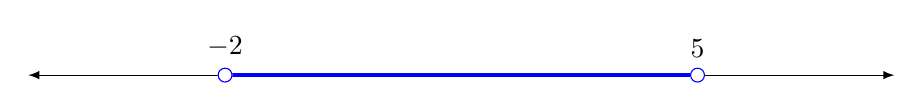
\begin{tikzpicture}
\draw[latex-latex] (-5.5,0) -- (5.5,0);
\draw[line width=1.5pt, color=blue] (-3,0) -- (3,0);
\filldraw[white](-3,0)circle[radius=2.5pt];
\draw[blue](-3,0)circle[radius=2.5pt];
\filldraw[white](3,0)circle[radius=2.5pt];
\draw[blue](3,0)circle[radius=2.5pt];
\node[at={(-3,3pt)},above]{$-2$};
\node[at={(3,3pt)},above]{$5$};
\end{tikzpicture}
\end{center}
空心圆 $\circ$ 表示端点不包含在区间内。
\end{example}

请注意，符号 $\infty$ 的使用具有误导性，因为它表明符号 $\infty$ 本身具有特定含义（或者更糟糕的是，它指的是实数）。实际上它不是实数 --- 它只是表明所讨论的区间为无界区间的符号。例如，$[a, \infty)$ 的一种较少误导性的书写方式可能是 $[a, {\to})$ 或 $\mathbb{R}^{\ge a}$；然而，$[a,\infty)$ 是标准，所以我们就要这么写。

\begin{exercise}
对于以下每个图示，找出它所描绘的区间。实心圆 $\bullet$ 表示该区间包含端点，而空心圆 $\circ$ 表示该区间不包含端点。

\begin{enumerate}[(a)]
\item
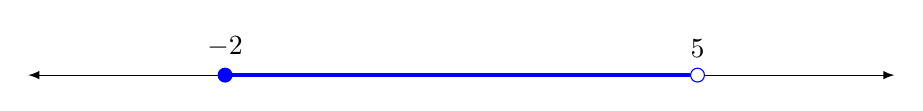
\begin{tikzpicture}
\draw[latex-latex] (-5.5,0) -- (5.5,0);
\draw[line width=1.5pt, color=blue] (-3,0) -- (3,0);
\filldraw[blue](-3,0)circle[radius=2.5pt];
\filldraw[white](3,0)circle[radius=2.5pt];
\draw[blue](3,0)circle[radius=2.5pt];
\node[at={(-3,3pt)},above]{$-2$};
\node[at={(3,3pt)},above]{$5$};
\end{tikzpicture}

\item
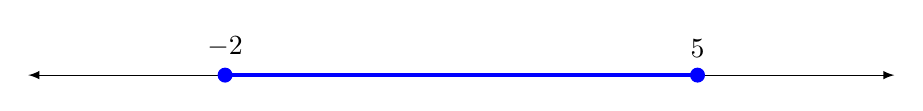
\begin{tikzpicture}
\draw[latex-latex] (-5.5,0) -- (5.5,0);
\draw[line width=1.5pt, color=blue] (-3,0) -- (3,0);
\filldraw[blue](-3,0)circle[radius=2.5pt];
\filldraw[blue](3,0)circle[radius=2.5pt];
\node[at={(-3,3pt)},above]{$-2$};
\node[at={(3,3pt)},above]{$5$};
\end{tikzpicture}


\item
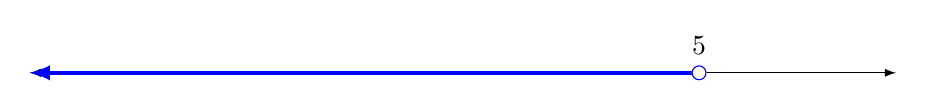
\begin{tikzpicture}
\draw[latex-latex] (-5.5,0) -- (5.5,0);
\draw[latex-, line width=1.5pt, color=blue] (-5.5,0) -- (3,0);
\filldraw[white](3,0)circle[radius=2.5pt];
\draw[blue](3,0)circle[radius=2.5pt];
\node[at={(3,3pt)},above]{$5$};
\end{tikzpicture}

\item 
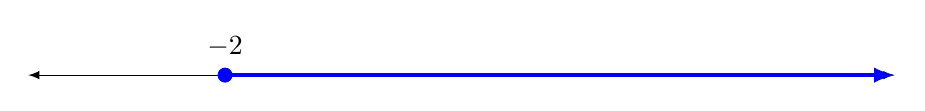
\begin{tikzpicture}
\draw[latex-latex] (-5.5,0) -- (5.5,0);
\draw[-latex, line width=1.5pt, color=blue] (-3,0) -- (5.5,0);
\filldraw[blue](-3,0)circle[radius=2.5pt];
\node[at={(-3,3pt)},above]{$-2$};
\end{tikzpicture}
\end{enumerate}
\end{exercise}

\subsection*{子集}

通常情况下，某个集合的所有元素也是另一个集合的元素。例如，每个整数都是有理数；即
\[ \forall n \in \mathbb{Z},\, n \in \mathbb{Q} \]
我们可以更简洁地说 $\mathbb{Z}$ 是 $\mathbb{Q}$ 的\textit{子集}。

\begin{definition}
\label{defSubset}
\index{subset}
设 $X$ 为一个集合。$X$ 的\textbf{子集}是一个集合 $U$，满足
\[ \forall a,\, (a \in U \Rightarrow a \in X) \]
我们用 $U \subseteq X$\nindex{subset}{$\subseteq$}{subset} \inlatex{subseteq}\lindexmmc{subseteq}{$\subseteq$} 来表示 $U$ 是 $X$ 的子集。

此外，符号 $U \nsubseteq X$ \inlatex{nsubseteq}\lindexmmc{nsubseteq}{$\nsubseteq$} 表示 $U$ 不是 $X$ 的子集，而符号 $U \subsetneqq X$ \inlatex{subsetneqq}\lindexmmc{subsetneqq}{$\subsetneqq$} 表示 $U$ 是 $X$ 的\textbf{真子集}，即 $X$ 的子集不等于 $X$。
\end{definition}

\begin{strategy}[证明子集包含]
要想证明集合 $U$ 是集合 $X$ 的子集，只需取任意元素 $a \in U$ 并证明 $a \in X$ 即可。
\end{strategy}

\begin{example}
每个集合都是其自身的子集 --- 即对于所有集合 $X$, $X \subseteq X$。这个证明非常简单：我们只须证明  $\forall x \in X,\, x \in X$。但这是显而易见的：假设 $x \in X$，则 $x \in X$。搞定！
\end{example}

\begin{example}
设 $a,b,c,d \in \mathbb{R}$ 且 $a<c<d<b$。则 $[c,d] \subseteq (a,b)$。事实上，让 $x \in [c,d]$。 则 $c \le x \le d$。因此
\[ a < c \le x \le d < b \quad \Rightarrow \quad a < x < b \]
所以 $[c,d] \subseteq (a,b)$。
\end{example}

\begin{exercise}
设 $a,b,c,d \in \mathbb{R}$ 其中 $a<b$ 且 $c<d$。证明 $[a,b) \subseteq (c,d]$ 当且仅当 $a > c$ 且 $b \le d$。
\end{exercise}

\begin{example}
\Cref{chGettingStarted} 中的数集通过以下子集包含链关联。
\[ \mathbb{N} \subseteq \mathbb{Z} \subseteq \mathbb{Q} \subseteq \mathbb{R} \subseteq \mathbb{C} \]
\end{example}

下面的命题证明了子集的\textit{传递性} --- 我们将在 \Cref{secRelations} 中重新审视这个性质。

\begin{proposition}
\label{propSubsetTransitive}
设 $X,Y,Z$ 为集合。如果 $X \subseteq Y$ 且 $Y \subseteq Z$，则 $X \subseteq Z$。
\end{proposition}

\begin{cproof}
假设 $X \subseteq Y$ 且 $Y \subseteq Z$。我们需要证明 $X \subseteq Z$。

设 $a \in X$。因为 $X \subseteq Y$, 根据 \Cref{defSubset} 可得 $a \in Y$；又因为 $Y \subseteq Z$，再次根据 \Cref{defSubset} 可得 $a \in Z$。

因此 $X \subseteq Z$。
\end{cproof}

\subsection*{集合相等}

本节主要讨论定义集合、比较集合以及从原集合构建新集合，因此为了取得更大进展，我们首先需要明确当我们说两个集合\textit{相等}时我们具体指什么。

\begin{discussion}
\label{dscSetEquality}
设 $X$ 和 $Y$ 为集合。$X$ 和 $Y$ 相等是什么意思？在继续阅读之前，尝试给出集合相等的精确定义。
\end{discussion}

集合的 `相同性' 可能有不同的概念：当两个集合 $X$ 和 $Y$ 具有完全相同的定义时，我们可能说它们相等；或者我们可能说，当 $X$ 和 $Y$ 包含相同的对象作为元素时，它们是相等的。例如，假设 $X$ 是 `所有奇自然数的集合'，而 $Y$ 是 `连续完全平方差的所有整数的集合' --- 在这种情况下，第一种说法可能会导致我们说 $X \ne Y$，而第二种说法会导致我们说 $X = Y$。

很明显，我们必须在适当的时候给出严格的定义。而现在正是时候。

\begin{axiom}[集合外延性]
\label{axSetEquality}
\index{set equality}
\index{extensionality}
设 $X$ 和 $Y$ 为集合。则 $X=Y$ 当且仅当 $\forall a,\, (a \in X \Leftrightarrow a \in Y)$，或等价地，如果 $X \subseteq Y$ 且 $Y \subseteq X$。
\end{axiom}

集合相等的这种特征给出了以下证明两个集合相等的策略。

\begin{strategy}[双重包含证明]
要想证明集合 $X$ 等于集合 $Y$，只需：
\begin{itemize}
\item 证明 $X \subseteq Y$，例如，设 $a \in X$ 为任意元素，然后推导出 $a \in Y$；
\item 证明 $Y \supseteq X$, 例如，设 $a \in Y$ 为任意元素，然后推导出 $a \in X$。
\end{itemize}
我们经常用 `($\subseteq$)' 和 `($\supseteq$)' 表示要证明的包含性的方向。
\end{strategy}

\begin{example}
\label{exPositiveNegativeSetBuilderNotation}
用双重包含证明 $\{ x \in \mathbb{R} \mid x^2 \le 1 \} = [-1,1]$。
\begin{itemize}
\item ($\subseteq$) 设 $a \in \{ x \in \mathbb{R} \mid x^2 \le 1 \}$。则 $a \in \mathbb{R}$ 且 $a^2 \le 1$ 所以 $(1-a)(1+a) = 1-a^2 \ge 0$。则有如下 2 种情况:
\begin{itemize}
\item $1-a \ge 0$ 且 $1+a \ge 0$，这种情况下 $a \le 1$ 且 $a \ge -1$，所以 $a \in [-1,1]$。
\item $1-a \le 0$ 且 $1+a \le 0$, 这种情况下 $a \ge 1$ 且 $a \le -1$, 这会引出矛盾 $-1 < 1$.
\end{itemize}
所以满足条件的只能是 $a \in [-1,1]$。

\item ($\supseteq$) 设 $a \in [-1,1]$。则 $-1 \le a \le 1$，所以 $|a| \le 1$，又因为 $a^2 = |a|^2 \le 1$，所以 $a \in \{ x \in \mathbb{R} \mid x^2 \le 1 \}$。
\end{itemize}
\end{example}

\begin{exercise}
证明 $\{ x \in \mathbb{R} \mid x^2 < x \} = (0,1)$。
\end{exercise}

集合外延性公理的结论是，集合与其元素在列表表示法中出现的顺序无关，并且与单个元素被写入的次数无关 --- 也就是说，集合的元素仅`计数'一次，即使它在列表表示法中出现多次。下面的练习对此进行了说明。

\begin{exercise}
用双重包含证明 $\{ 0, 1 \} = \{ 1, 0 \}$ 且 $\{ 0, 0 \} = \{ 0 \}$。
\end{exercise}

\subsection*{空集和非空集}

集合的另一个基本示例是\textit{空集}，即没有任何元素的特定集合。这里我们必须留意`特定'这个词，因为它意味着\textit{唯一性}，而且我们（还）不知道两个没有元素的集合一定是相等的。因此，首先我们将定义空集的含义，然后我们将证明只有一个空集。

\begin{definition}
\label{defInhabited}
\label{defEmptyProperty}
\index{empty set}
\index{set!empty}
\index{inhabited set}
\index{set!inhabited}
如果集合 $X$ 至少有一个元素，则该集合是\textbf{有元的（inhabited）}（或\textbf{非空的（nonempty）}）；否则，它就是\textbf{空的（empty）}。
\end{definition}

集合 $X$ 非空的断言等价于逻辑公式 $\exists a,\, a \in X$，而集合 $X$ 为空的断言等价于逻辑公式 $\neg \exists a,\, a \in X$。这表明可以采用以下策略来证明一个集合是空集还是非空集。

\begin{strategy}[证明集合是空集还是非空集]
要想证明集合 $X$ 是非空集，只要展示一个元素即可。为了证明集合 $X$ 是空集，假设 $X$ 是非空集 --- 也就是说，存在某个元素$a \in X$ --- 并导出矛盾。
\end{strategy}

其他教科书中，术语\textit{非空（nonempty）}比\textit{有元（inhabited）}更常见，但有理由更喜欢后者。事实上，语句`$X$ 是非空的'更直接地翻译为 $\neg(\neg \exists a,\, a \in X)$，它有一个不必要的双重否定，并暗示了通过矛盾来证明。因此，我们在本书中使用术语 \textit{有元（inhabited）}。

为空似乎是一种微不足道的状况 --- 事实确实如此 --- 但由于它的经典性，它无处不在。

\begin{example}
集合 $\{ x \in \mathbb{R} \mid x^2 = 2 \}$ 非空，例如 $\sqrt{2} \in \mathbb{R}$ 且 $\sqrt{2} ^2 = 2$。然而，集合 $\{ x \in \mathbb{Q} \mid x^2 = 2 \}$ 为空，因为如果非空，则存在一个有理数 $x$ 使得 $x^2 = 2$，而这与 \Cref{propSqrt2IrrationalPreliminary} 矛盾。
\end{example}

\begin{example}
我们在 \Cref{exBracketN} 中观察到集合 $[0]$ 为空；这是一个更正式的证明。为了引出矛盾，我们假设 $[0]$ 非空。则存在某些 $k \in \mathbb{N}$ 使得 $1 \le k \le 0$。由此可得 $1 \le 0$，这与 $0<1$ 的事实相矛盾。 因此 $[0]$ 一定为空。
\end{example}

\begin{exercise}
设 $a,b \in \mathbb{R}$。证明 $[a,b]$ 为空，当且仅当 $a > b$; $(a,b)$ 为空，当且仅当 $a \ge b$。
\end{exercise}

下一个练习涉及细致的逻辑技术，它有些反直觉，与爆炸原理（\Cref{axPrincipleOfExplosion}）难以掌握的原因相同。然而，它对于证明空集的事实非常有用，我们很快就会在 \Cref{thmEmptySetIsUnique} 中看到。

\begin{exercise}
设 $E$ 为空集，并设 $p(x)$ 为具有一个自由变量 $x$ 且论域为 $E$ 的谓词。证明命题 $\forall x \in E,\, p(x)$ 为真，命题 $\exists x \in E,\, p(x)$ 为假。命题 $\forall x \in E,\, x \ne x$ 在中文里是什么意思？这是真的吗？
\hintlabel{exEverythingIsTrueOfElementsOfEmptySet}{%
回想一下 \Cref{secSets} 的开头，$\forall x \in X,\, p(x)$ 等价于 $\forall x,\, (x \in X \Rightarrow p(x))$ 并且 $\exists x \in X,\, p(x)$ 等价于 $\exists x,\, (x \in X \wedge p(x))$。当 $E$ 为空时，$x \in E$ 的真值可以怎么说？
}
\end{exercise}

由于外延性公理 (\Cref{axSetEquality})，任何两个空集都必须相等，因为它们都包含相同的元素 --- 即根本没有元素！以下定理给出了正式阐述。

\begin{theorem}
\label{thmEmptySetIsUnique}
设 $E$ 和 $E'$ 为集合。如果 $E$ 和 $E'$ 为空，则 $E=E'$。
\end{theorem}
\begin{proof}
假设 $E$ 和 $E'$ 为空集。断言 $E=E'$ 等价于
\[ (\forall a \in E,\, a \in E') \wedge (\forall a \in E',\, a \in E) \]
因为 $E$ 和 $E'$ 为空集，根据 \Cref{exEverythingIsTrueOfElementsOfEmptySet}，$\forall a \in E,\, a \in E'$ 和 $\forall a \in E',\, a \in E$ 均为真。所以 $E=E'$。
\end{proof}

知道只有一个空集意味着我们现在可以做出以下定义，而不必担心`特定'这个词是否有问题。

\begin{definition}
\label{defEmptySet}
\nindex{O}{$\varnothing$}{empty set}
\index{empty set}
\index{set!empty}
\textbf{空集}（也叫 \textbf{null集}）是没有元素的集合，用 $\varnothing$ \inlatex{varnothing}\lindexmmc{varnothing}{$\varnothing$} 表示。
\end{definition}

有些作者将空集写做 $\{ \}$ 而不是 $\varnothing$，那是因为 $\{ \}$ 是用列表表示法表示的空集。

\begin{exercise}
\label{exEmptySetSubsetOfEverySet}
设 $X$ 是一个集合。证明 $\varnothing \subseteq X$。
\end{exercise}

\subsection*{幂集}

\begin{definition}
\label{defPowerSet}
\index{power set}
设 $X$ 为一个集合。$X$ 的 \textbf{幂集}，写作 $\mathcal{P}(X)$\nindex{PX}{$\mathcal{P}(X)$}{power set} \inlatex{mathcal\{P\}}\lindexmmc{mathcal}{$\mathcal{A}, \mathcal{B}, \dots$} 是 $X$ 所有子集的集合。
\end{definition}

\begin{example}
$\{ 1, 2 \}$ 有四个子集，即
\[ \varnothing, \quad \{ 1 \}, \quad \{ 2 \}, \quad \{ 1, 2 \} \]
所以 $\mathcal{P}(X) = \{\varnothing, \{ 1 \}, \{ 2 \}, \{ 1, 2 \}\}$。
\end{example}

\begin{exercise}
写出 $\mathcal{P}(\{1, 2, 3\})$ 的所有元素。
\end{exercise}

\begin{exercise}
设 $X$ 为一个集合。证明 $\varnothing \in \mathcal{P}(X)$ 且 $X \in \mathcal{P}(X)$。
\end{exercise}

\begin{exercise}
写出 $\mathcal{P}(\varnothing)$, $\mathcal{P}(\mathcal{P}(\varnothing))$ 和 $\mathcal{P}(\mathcal{P}(\mathcal{P}(\varnothing)))$ 的所有元素。
\end{exercise}

幂集常常是一个令人困惑的点，因为它们将一个集合的\textit{子集}带到另一个集合的\textit{元素}中，从某种意义上说，对于所有集合 $U$ 和 $X$ 我们有
\[ U \subseteq X \quad \Leftrightarrow \quad U \in \mathcal{P}(X) \]
这种区别看起来很容易掌握，但是当集合 $U$ 和 $X$ 看起来很相似时，很容易陷入各种陷阱。这里有一个简单的例子。

\begin{example}
$\varnothing \subseteq \varnothing$ 为真，但 $\varnothing \in \varnothing$ 为假。的确，
\begin{itemize}
\item $\varnothing \subseteq \varnothing$ 意味着 $\forall x \in \varnothing,\, x \in \varnothing$；如 \Cref{exEverythingIsTrueOfElementsOfEmptySet} 中所述，$\forall x \in \varnothing,\, p(x)$ 形式的命题始终为真。
\item 空集没有元素；如果 $\varnothing \in \varnothing$ 为真，则意味着 $\varnothing$ 有一个元素（该元素是 $\varnothing$）。所以情况一定是 $\varnothing \not \in \varnothing$。
\end{itemize}
\end{example}

以下练习旨在帮助您通过练习克服类似的潜在困惑。尝试精确思考所涉及的定义是什么。

\begin{exercise}
通过证明判断以下每项陈述是否正确。
\begin{enumerate}[(a)]
\item $\mathcal{P}(\varnothing) \in \mathcal{P}(\mathcal{P}(\varnothing))$;
\item $\varnothing \in \{ \{ \varnothing \} \}$;
\item $\{ \varnothing \} \in \{ \{ \varnothing \} \}$;
\item $\mathcal{P}(\mathcal{P}(\varnothing)) \in \{ \varnothing, \{ \varnothing, \{ \varnothing \} \} \}$.
\end{enumerate}
重复以上练习，将 `$\in$' 全部替换为 `$\subseteq$'。
\end{exercise}

\begin{tldr}{secSets}

\subsubsection*{集合与子集}

\begin{tldrlist}
\tldritem{defSet} \textit{集合}是来自固定\textit{论域} $\mathcal{U}$ 的对象（称为\textit{元素}）的汇集；写做 $x \in X$ 表示 $x$ 是集合 $X$ 的一个元素。集合可以通过（显式或隐式）列出其元素 $\{ x_1, x_2, \dots, x_n, \dots \}$ 或使用\textit{集合构建表示法}来指定。
\tldritem{defSubset} 如果 $\forall a,\, (a \in U \Rightarrow a \in X)$，则集合 $U$ 是集合 $X$ 的\textit{子集}，写作 $U \subseteq X$。为了证明 $U \subseteq X$，只需引入一个变量 $a$，假设 $a \in U$，并推导出 $a \in X$。
\tldritem{axSetEquality} 集合 $X$ 和 $Y$ 相等，当且仅当 $\forall a,\, (a \in X \Leftrightarrow a \in Y)$。为了证明 $X = Y$，只需分别证明 $X \subseteq Y$ 且 $Y \subseteq X$ 即可 --- 这种方法称为\textit{双重包含}。
\end{tldrlist}

\subsubsection*{空集和非空集}

\begin{tldrlist}
\tldritem{defInhabited} 一个集合 $X$ 如果至少有一个元素，则是\textit{非空的}；否则，便是\textit{空的}。
\tldritem{thmEmptySetIsUnique} 只有唯一一个空集，用 $\varnothing$ 或 $\{ \}$ 表示。
\end{tldrlist}

\subsubsection*{幂集}
\begin{tldrlist}
\tldritem{defPowerSet} 集合 $X$ 的\textit{幂集}是 $X$ 所有子集的集合。
\end{tldrlist}
\end{tldr}